\chapter{Pulse Width} 
\lstset{style=6502Style}

\begin{figure}[H]
    \centering
    \begin{adjustbox}{width=10.5cm,margin=0cm}
      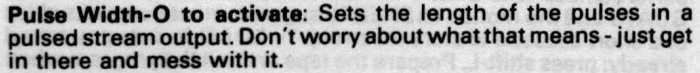
\includegraphics[width=12cm]{src/pulsewidth/pulsewidth.png}%
    \end{adjustbox}
    \caption{
      Excerpt from Manual (Part No. LC1982-Vb). Pulse Width.
      }
\end{figure}

\begin{lstlisting}[caption=From \icode{CheckKeyboardInput}.]
MaybeOPressed   
        CMP #KEY_O ; O pressed.
        BNE MaybeAsteriskPressed

        ; O pressed.
        ; Pulse Width : Sets the length of the pulses in a pulsed
        ; stream output. Don't worry about what that means - just get in there
        ; and mess with it.
        LDA #PULSE_WIDTH
        STA currentVariableMode
        RTS 
\end{lstlisting}

\begin{figure}[H]
    \centering
    \begin{adjustbox}{width=3cm,margin=11cm -12cm}
      
\includegraphics[width=12cm]{src/pulsewidth/pulsewidth-low.png}%
    \end{adjustbox}
    \begin{adjustbox}{width=10.5cm,center}
      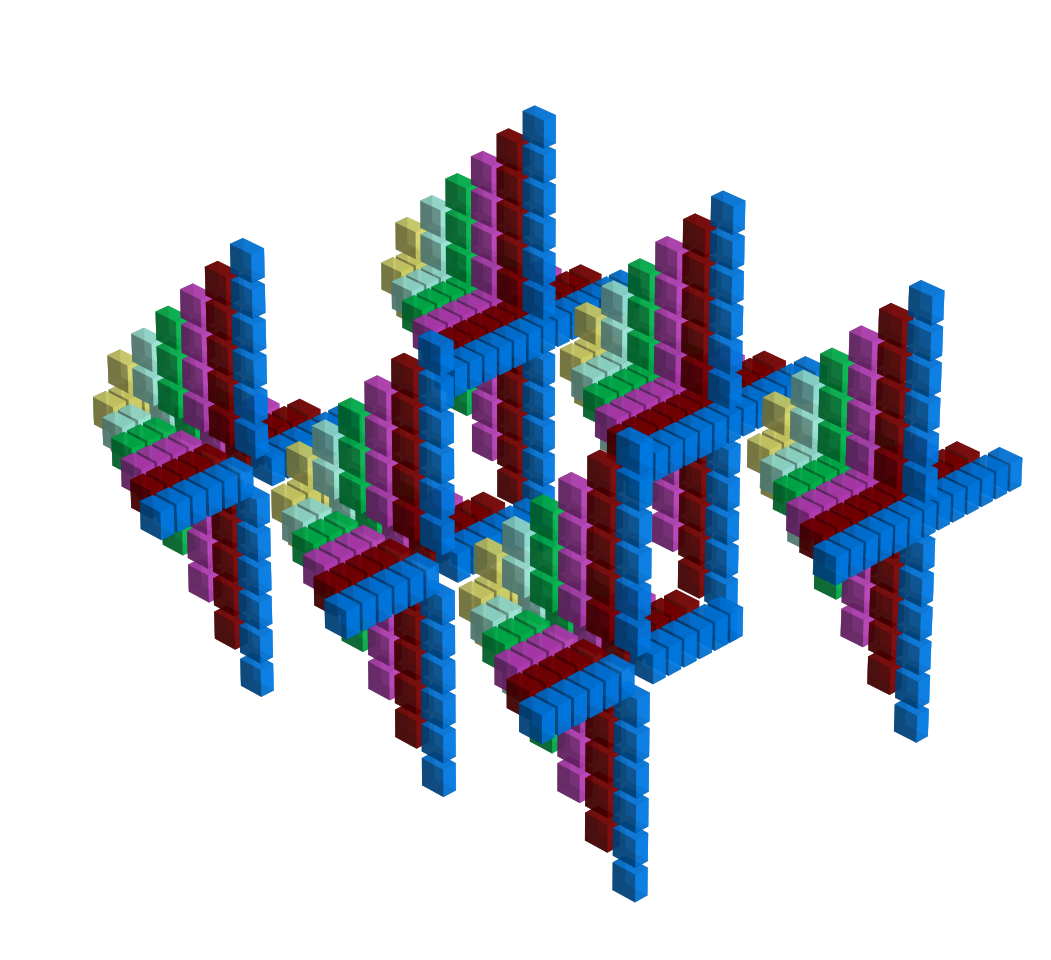
\includegraphics[width=12cm]{src/pulsewidth/pattern0-45.png}%
    \end{adjustbox}
    \begin{adjustbox}{width=3cm,margin=11cm -12cm}
      
\includegraphics[width=12cm]{src/pulsewidth/pulsewidth-high.png}%
    \end{adjustbox}
    \begin{adjustbox}{width=10.5cm,margin=0cm -2cm}
      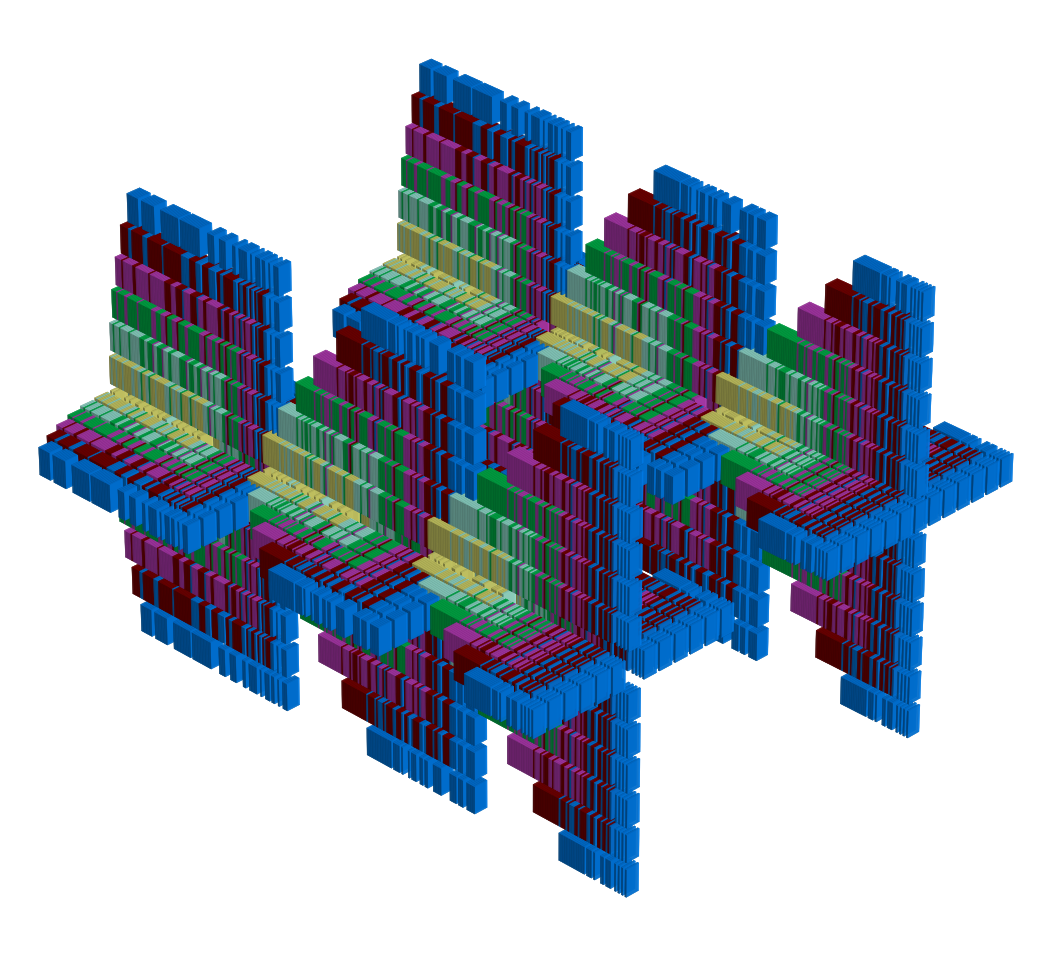
\includegraphics[width=12cm]{src/pulsewidth/pattern1-45.png}%
    \end{adjustbox}
    \caption{Effect of low and high values for Pulse Width}
\end{figure}


\begin{lstlisting}[caption=From \icode{CheckKeyboardInputForActiveVariable}. Pressing the < and > keys increments and
decrements the value in presetValueArray pointed to by \icode{X}\, i.e. \icode{currentVariableMode}.]
UpdateVariableDisplay   
        LDA #>SCREEN_RAM + $03D0
        STA colorBarColorRamHiPtr
        LDA #<SCREEN_RAM + $03D0
        STA colorBarColorRamLoPtr

        LDX currentVariableMode
        LDA lastKeyPressed
        CMP #$2C ; > pressed?
        BNE MaybeLeftArrowPressed

        ; > pressed, increase the value bar and write
        ; it to the approiate place in presetValueArray
        INC presetValueArray,X
        LDA presetValueArray,X
        ; Make sure we don't exceed the max value.
        CMP maxValueForPresetValueArray,X
        BNE MaybeInColorMode
        DEC presetValueArray,X
        JMP MaybeInColorMode
\end{lstlisting}

\begin{lstlisting}[caption=From \icode{ActivateSequencer}.]
; This is where the presets get loaded to. It represents
; the data structure for the presets.
; currentVariableMode is an index into this data structure
; when the user adjusts settings.
presetValueArray
unusedPresetByte        .BYTE $00
smoothingDelay          .BYTE $0C
cursorWidth             .BYTE $02
bufferLength            .BYTE $1F
pulseWidth              .BYTE $01; <-- Pulse Width is here at position \icode{\$04}.
indexForColorBarDisplay .BYTE $01
lineWidth               .BYTE $07
sequencerWidth          .BYTE $04 
pulseWidth              .BYTE $01
baseLevel               .BYTE $07
presetColorValuesArray  .BYTE BLACK,BLUE,RED,PURPLE,GREEN,CYAN,YELLOW,WHITE
trackingActivated       .BYTE $FF
lineModeActivated       .BYTE $00
presetIndex            .BYTE $05
\end{lstlisting}


\begin{lstlisting}[caption=From \icode{MainInterruptHandler}.]
DecrementPulseWidthCounter   
        DEC currentPulseWidthCounter
        BEQ RefreshPulseWidth
        JMP DrawCursorAndReturnFromInterrupt
        ; Returns

RefreshPulseWidth   
        LDA pulseWidth
        STA currentPulseWidthCounter
        LDA pulseWidth
        STA currentPulseWidth
\end{lstlisting}
